\begin{ZhChapter}

\chapter{研究方法}

\section{研究架構與整體流程}

\text 本章節根據文獻探討對於RESTLess混合優化策略,與本研究提出的自動化測試框架採用創新的分散式雙主機架構(Distributed Dual-Host Architecture)融合,其核心優勢在於實現責任隔離與協議互操作性。基於對A2A協定和MCP協定的雙協定整合的流程設計,RESTLess的兩大優化策略將分別應用於不同的代理人(Agent)和階段,以最大化LLM的專業分工和雙協定(A2A與MCP)的優勢,旨在克服傳統單一LLM代理框架在上下文一致性和跨主機任務協調方面的挑戰。整體流程圍繞五大關鍵階段展開,從接收測試需求開始,透過代理間的結構化通訊和專業工具整合,最終輸出完整的測試報告,並自動化銜接CI/CD流程中的Git操作。
\text 首先,由Planner Agent啟動流程,將OpenAPI JSON輸入檔及Manual Document,透過呼叫FastMCP服務作為外部工具知識庫進行執行資料處理及垂直整合;接著,針對回傳的測試條件後,由Planner Agent使用A2A協定的任務委派模式,將生成測試腳本的任務傳遞給Test Coder Agent及Executor Agent進行腳本生成與執行;第三階段為結果分析與自校準,Executor Agent將原始的執行結果(包括HTTP狀態碼狀態碼2XX/4XX/5XX),透過A2A協定回傳給Analyzer Agent,若失敗時會啟動Re-loop流程,將失敗原因和當前狀態,回饋給Planner Agent,並指派Test Coder Agent進行修復性代碼生成;最後,進而再次呼叫FastMCP服務,啟動Reporter Agent執行外部操作(GitOps),完成最終報告生成與結案,並發送A2A請求給位於Host 2上的GitOps Agent,允許代理跨越協議邊界進行協作。

\subsection{主機劃分與角色分配}

\text 本研究提出了一個高度模組化且具備跨系統協作能力的自動化測試生成與驗證框架。此框架的核心理念是結合A2A協定實現代理間的任務協調與狀態傳遞,並透過MCP協定實現上下文感知的專業工具服務。整個系統由兩個邏輯隔離的主機和六個專業代理共同驅動。
\text 本架構由兩組獨立的主機環境組成,整體流程涵蓋四個主要大角色與協定任務:AutoGen Host、FastMCP Client、FastMCP Server、External A2A Host、GitOps Host,以及六個代理Agents與子任務: Planner Agent、Test Coder Agent、Executor Agent、Analyzer Agent、Reporter Agent、GitOps Agent,,以達成功能隔離和安全分權,以下為詳細分權及說明:
\begin{enumerate}
    \item Host 1:AutoGen A2A Host (測試與分析主機)
    \begin{itemize}
        \item 角色定位: 作為主要的A2A 控制中心和 FastMCP Client,負責整個測試流程的生命週期管理。
        \item 組成與任務: 包含 Planner Agent、Test Coder Agent、Executor Agent、Analyzer Agent 四個核心 Agent。它也是 FastMCP Server 的物理部署位置,並在內部以 LangChain 庫的形式提供專業的 MCP 工具服務(例如:API Item 前置處理、報告生成)。
        \item 協議職責: 主導 Host 1 內部 Agent 間的 A2A 協作,並作為 A2A Client 向 Host 2 的 External A2A Host 發送跨主機請求。
    \end{itemize}
    \item Host 2:External A2A Host / GitOps Host (部署與操作主機)
    \begin{itemize}
        \item 角色定位: 作為 A2A Server,專門接收來自 Host 1 的高權限操作請求,實現安全隔離。
        \item 組成與任務: 僅包含 GitOps Agent。該 Agent 負責對 SUT (System Under Test) 的 Git Repository 執行所有 Git 操作,例如版本標記(Tag)、分支合併(Merge)等。
        \item 協議職責: 透過 A2A 介面接收 Host 1 的任務,執行 GitOps 流程,並將操作的成功或失敗狀態回傳給 Host 1,確保了測試與部署環境的權責分離。
    \end{itemize}
\end{enumerate}

\subsection{自動化測試生成與驗證流程概述}
\text 整個自動化流程是一套由A2A協議驅動的閉環(Closed-Loop)協作,其中MCP協議在關鍵節點提供專業能力與上下文一致性。各階段間之互動說明如下:
\subsubsection*{階段(一)輸入與前置處理(Input \& Pre-processing)}
\text 本階段將以接收使用者提供的OpenAPI JSON檔案(定義測試目標)與Manual Document(包含預期結果及操作步驟等,作為高語義測試案例)。整體服務流程由Planner Agent啟動,透過呼叫FastMCP(由LangChain程式庫支持的工具互動層),執行API item的資料處理與分類。此MCP服務中將嵌入LLM-Based Specification Semantic Optimization模組(類似RESTLess的語義增強演算法)。處理後的分類結果和Manual Document(包含人類預期結果)一同被封裝成核心上下文(Core Context),作為A2A狀態資料結構的一部分,注入到測試流程中。

\subsubsection*{階段(二)腳本生成與執行(Code Generation \& Execution)}
\text 接繼使用A2A協定的任務委派模式,將生成測試腳本的任務傳遞給Test Coder Agent,依據A2A狀態資料中包含的MCP Context(即語義增強後的規格),實施Weight-Based Render Order Optimization策略(類似RESTLess的渲染順序優化)。
\text 然後,透過機率ω調整 來決定是否添加低權重(Non-Required)參數進行測試,從而生成更長、更多樣化的測試序列,以檢測隱藏在複雜操作組合中的錯誤。腳本隨後被傳遞給Executor Agent,執行針對測試目標進行RESTful API的黑箱測試。

\subsubsection*{階段(三)結果分析與自校準(Analysis \& Self-Correction)}
\text 在此階段,Executor Agent及Analyzer Agent扮演自動化測試流程驗證與修正的重要橋樑,流程如下:
\begin{enumerate}
    \item Executor Agent將原始的執行結果(包括 HTTP 狀態碼 20X/50X)透過A2A協定回傳給Analyzer Agent。
    \item Analyzer Agent利用Manual Document提供的預期結果進行結果比對(即測試案例),判斷測試成功或失敗。
    \begin{itemize}
        \item Re-loop機制(自校準):若失敗,Analyzer Agent將失敗原因和當前狀態(維持在 MCP Context中)回饋給Planner Agent。Planner Agent啟動Re-loop流程,指派Test Coder Agent進行修復性代碼生成,直至測試成功。
    \end{itemize}
\end{enumerate}

\subsubsection*{階段(四)CI/CD外部操作(GitOps Integration)}
\text 階段(三),一旦測試成功,Executor Agent(類似於IT事件響應系統中報告解決狀態的代理)發送A2A請求給GitOps Host的GitOps Agent。此實施展現了雙協定的互通性,允許代理跨越協議邊界進行協作。
\text GitOps Agent接收A2A結構化請求後,執行相關的Git操作(例如打Tag、Merge Branch或Pull Request),實現從測試到部署的自動化銜接。

\subsubsection*{階段(五)報告生成與結案(Reporting \& Closure)}
\text 最後,Analyzer Agent回傳資料給Planner Agent後將再次呼叫FastMCP服務,啟動Reporter Agent。透過MCP協定的上下文感知層,存取並整合整個A2A流程的所有日誌、執行結果、Manual Document的預期值,以及前置處理的分類結果。MCP在此階段確保了所有工具和代理在整個複雜流程中上下文的一致性,最終生成一份完整且結構化的最終測試報告。

\section{前置處理的理論與設計}
\text 為建構具備高語義品質的核心上下文(Core Context),此上下文對於後續代理(Agent)生成有效且能通過雲端閘道檢查的測試腳本至關重要。本階段的設計核心,在於整合模型上下文協議(MCP)的垂直整合優勢,以及源於RESTLess框架的語義優化策略。

\text 此階段的理論基礎聚焦於克服僅依賴原始OpenAPI規範作為測試輸入的侷限性。傳統的 REST API 模糊測試(Fuzzing)方法,其挑戰在於生成的請求序列普遍缺乏業務語義價值,從而導致大量的語義缺失請求在雲端閘道層被語法或業務邏輯檢查所阻擋,嚴重影響測試效率。
\text 為解決此問題,本研究引入MCP作為上下文感知層(Contextual Awareness Layer),以確保跨Agent與工具間的語義一致性。Planner Agent作為FastMCP Client,透過呼叫FastMCP Server(其工具互動層由LangChain程式庫提供支持),實現對規格數據和人類知識的安全且一致性存取。此外,我們整合了基於LLM的規格語義優化模組(LLM-Based Specification Semantic Optimization),此模組旨在增強原始OpenAPI規範的語義豐富度,進而提升有效請求序列的通過率。

\text 本階段的實施流程旨在將非結構化或半結構化輸入轉化為高語義的結構化上下文,其步驟如下:
\text 系統首先接收兩類輸入:OpenAPI JSON檔案(定義API結構與參數名稱)和Manual Document(包含高語義測試案例、預期結果及操作步驟等)。由Planner Agent隨即透過A2A協定發出任務,並作為FastMCP Client呼叫FastMCP服務,以執行API item的資料處理與分類。
\text 在 FastMCP 服務內部,嵌入的 LLM-Based Semantic Optimization 模組執行語義增強演算法:

\begin{enumerate}
    \item 模組透過精確的 Prompt Engineering,指示底層 LLM 學習原始規範中參數的潛在語義(例如,從名稱判斷用途),並生成多個語義相似且具代表性的參數值集合(RTSet)。
    \item 緊接著,LLM 自動掃描原始 OpenAPI 規範,將生成的 para-value 鍵值對從 RTSet 替換或補充到對應參數的 enum 字段中。此步驟旨在確保 Test Coder Agent 能夠存取到具備業務語義的有效輸入值,而非隨機生成的無效數據。
\end{enumerate}

\text 經過FastMCP服務處理後,最終的輸出結果(包括分類結果、語義增強後的規格,以及Manual Document中包含的人類預期結果)將被標準化封裝成核心上下文(Core Context)。此核心上下文作為A2A狀態資料結構的一部分,被注入到測試流程中。此機制確保了後續的Test Coder Agent在生成腳本時,能夠在語法和語義上都依據一個一致且強化過的測試依據,從而大幅提升測試腳本的準確率和有效性。

\text 本研究建議利用LangChain程式庫作為FastMCP服務中的底層工具互動層。LangChain的Tool抽象機制用於將「OpenAPI語義增強」定義為一個可供Agent安全呼叫的服務。該Tool內部利用LangChain的LLM Chain執行所有Prompt Engineering和數據擴增邏輯。FastMCP服務在此充當上下文管理器,負責將LLM生成的高語義參數值安全地寫入到核心上下文中,確保Planner Agent透過MCP呼叫此服務時,能夠獲得上下文完整性的保證。

\begin{table*}[htbp]
    \centering
    \caption{語義優化與上下文建立範例設計對照表} 
    \label{tab:context_optimization}
    \scriptsize % 字體縮小
    \renewcommand{\arraystretch}{1.5} % 增加行距,讓沒格線的表格更好讀
    
    % 修改處:移除了直向分隔線 "|"
    % 使用 p{寬度} 確保中文自動換行且不報錯
    \begin{tabular}{p{2.5cm} p{6.5cm} p{6.5cm}}
        \toprule % 頂部粗線
        \textbf{Step} & \textbf{Content} & \textbf{Example} \\
        \midrule % 中間分隔線
        
        % 第 1 列
        輸入:原始規格 & 
        OpenAPI 規範:id 參數的類型為 \texttt{string},但無 \texttt{enum} 字段。 & 
        缺乏語義,可能被 Fuzzer 隨機填入 "123" 或 "abc",難以通過語義檢查。 \\
        \addlinespace % 增加列之間的空隙
        
        % 第 2 列
        輸入:Manual Document & 
        預期結果:"系統應接受格式為 U\_XXXXXX (X為數字) 的使用者 ID。" & 
        提供了高語義的有效值格式。 \\
        \addlinespace
        
        % 第 3 列
        MCP 服務執行語義優化 & 
        Planner Agent 呼叫 FastMCP 服務執行 LLM 數據擴增(類似 RESTLess)。 & 
        透過 Prompt 告訴 LLM id 的語義應是 U\_XXXXXX 格式。LLM 生成 RTSet 範例:["U\_001234", "U\_987654", "U\_555555"]。 \\
        \addlinespace
        
        % 第 4 列
        生成語義增強規格 & 
        FastMCP 服務將 RTSet 寫入規格的 \texttt{enum} 字段。 & 
        新的 OpenAPI 規範:id 參數新增 \texttt{enum}:["U\_001234", "U\_987654", "U\_555555"]。 \\
        \addlinespace
        
        % 第 5 列
        上下文封裝 & 
        Planner Agent 將增強後的規格和 Manual Document 封裝。 & 
        A2A 狀態資料結構中包含:\{API\_SPEC\_ENHANCED:<增強後規格>, EXPECTED\_RESULT:"系統應接受...",...\}。 \\
        
        \bottomrule % 底部粗線
    \end{tabular}
\end{table*}

這個強化後的上下文隨後被注入到A2A流程中,供Test Coder Agent在階段二進行腳本生成時使用,確保生成的測試請求在語法和語義上都具有高通過率。

\section{腳本生成與執行方法設計}
\text 此階段的設計依託於多代理系統的結構化任務委派能力,並融合了參照RESTLess框架的混合語義優化策略,旨在生成具備高效率和高覆蓋率的黑箱測試案例。
\text 將第一階段建構的語義強化上下文(MCP Context)轉化為可執行的測試序列的關鍵環節。主要奠基於A2A協議的水平協作特性,以及LLM驅動的語義優化,以突破傳統測試工具在處理RESTful API間複雜操作依賴和長序列生成上的技術瓶頸。

\subsection{測試腳本生成}
\text 流程始於Planner Agent透過A2A協定(由Autogen框架支持)啟動任務委託模式,將測試生成的任務與完整的A2A狀態資料(包含來自MCP服務的高語義化上下文)傳遞給Test Coder Agent。
\text A2A協定在此提供了標準化的訊息傳遞框架,確保了任務目標、上下文資訊和依賴圖(ODG)要求的清晰、無損傳遞,為腳本生成提供了穩定的輸入依據。

\text Test Coder Agent的生成是基於RESTLess的權重參數渲染順序優化策略 (Weight-Based Render Order Optimization),此策略旨在平衡測試序列的有效性(Validity)與多樣性(Diversity)。該策略首先根據API規範,將參數區分為高權重參數(例如Required必填欄位)和低權重參數(例如Non-required可選欄位)。高權重參數被視為確保請求序列符合語法與業務邏輯、能夠通過雲端閘道檢查的關鍵要素。優先使用高權重參數和階段一語義增強後的RTSet資料進行渲染,以確保生成的初始測試序列$S_1$具備高成功率。同時,Agent必須嚴格遵循操作依賴圖(ODG)的順序要求,確保前置操作的輸出(例如Session Token或ID)被正確擷取並注入為後續操作的輸入。在完成有效序列生成後,Test Coder Agent根據可靈活調整的機率$\omega$(例如預設值$\omega=80\%$),決定是否將低權重參數納入測試序列。此機率抽樣機制有效地擴展了測試案例的多樣性,增加了發現潛在邊緣錯誤(Edge Cases)的可能性,同時保持了對語義有效性的高度關注。

\subsection{腳本執行與黑箱測試驗證}
\text 生成的測試腳本(例如Python腳本)隨後被傳遞給Executor Agent執行。Executor Agent執行針對測試目標RESTful API的黑箱測試。其操作不依賴服務的內部原始碼,而是完全根據語義增強後的OpenAPI規範和Manual Document中的預期輸出來驗證系統的外部行為。
\text Executor Agent負責實際的HTTP請求發送,並準確記錄所有執行細節和原始結果(Raw Result),包括但不限於HTTP狀態碼(2XX, 4XX, 5XX)和回應主體。這些原始結果隨後透過A2A協定傳遞給下一階段的Analyzer Agent,作為結果分析與自校準的基礎輸入。

\text 透過上述設計,本階段確保了測試腳本不僅具備LLM的靈活性,更結合了工程的嚴謹性,為後續的自動化驗證與CI/CD流程奠定了高效且可靠的基礎。

\section{結果分析與自校準驗證機制設計}
\text 為應對整個自動化測試流程中驗證(Verification)回復(Recovery)錯誤復原(Error Recovery)結果分析與自校準驗證機制,此階段結合了A2A協定的訊息交換(Message Exchange)MCP Context所提供的上下文一致性,以實現高度自主的測試流程。
\text 本研究於此階段承繼Executor Agent的原始執行結果(即測試執行過程中產生的Artifacts透過A2A協定回傳給Analyzer Agent,包括 HTTP 狀態碼)判斷測試成功或失敗,決定是否啟動Re-loop機制。

\text 當Analyzer Agent判斷測試失敗後,它會將結構化(例如JSON或Topic-tagged tokens)的失敗原因和當前狀態透過A2A協定回饋給Planner Agent。這種回饋方式類似於ReAct 框架中的反思(Reflection)過程,確保錯誤診斷信息(例如,操作間依賴性錯誤或服務端邏輯錯誤)能夠被清晰地傳遞。
\text 在Re-loop過程中,MCP協議扮演了關鍵的上下文連續性角色。所有關鍵的當前狀態資訊(例如,導致失敗的參數序列、錯誤的執行堆疊)必須被安全且一致地維持在MCP Context中。這確保了在多步驟操作中,Planner Agent和Test Coder Agent能夠以一致的視角存取所需的診斷資訊,避免狀態遺失。
\text Planner Agent收到結構化回饋後,啟動Re-loop流程,並將修復任務重新委派給Test Coder Agent。此循環(規劃-執行-分析-修復)賦予了系統強大的強韌性,使其能夠在無需人工干預的情況下,透過反覆迭代優化其行動和計畫。

\begin{table*}[htbp]
    \centering
    \caption{範例應對表:處理參數依賴性錯誤} 
    \label{tab:dependency_error_handling}
    \scriptsize 
    \renewcommand{\arraystretch}{1.5} 
    
    % 去掉 "|",使用 p{寬度} 控制排版
    \begin{tabular}{p{2.5cm} p{6.5cm} p{6.5cm}}
        \toprule
        \textbf{Step} & \textbf{Content} & \textbf{Error \& Repair} \\
        \midrule
        
        Executor 執行 & 
        Executor Agent 執行腳本,但步驟(2)失敗,返回 404 Not Found。 & 
        A2A 傳輸結果:Executor Agent 將 404 狀態碼和堆疊追蹤作為 Artifacts 傳輸給 Analyzer Agent。 \\
        \addlinespace
        
        Analyzer 分析 & 
        Analyzer Agent 透過 LLM 檢查 Manual Document,發現預期結果應為 200 OK。分析結果的 404 狀態碼,與步驟(1)的輸出 user\_id 不一致,判斷測試失敗。 & 
        MCP Context 標記:Analyzer Agent 將失敗原因標記為:ERROR\_TYPE:Inter-operation Dependency Failure,並將此標記和當前 user\_id 的值維持在 MCP Context 中。 \\
        \addlinespace
        
        Planner 重新規劃 & 
        Planner Agent 接收到結構化失敗訊息和上下文後,啟動 Re-loop,並重新委派 Test Coder Agent。 & 
        Test Coder Agent 修復:代理意識到 user\_id 可能在步驟(1)中未被正確提取或格式化。它存取 MCP Context 中的資訊,修改腳本以確保 user\_id 被正確解析和注入到步驟(2)的 URL 中,直到測試成功。 \\
        \addlinespace
        
        生成語義增強規格 & 
        FastMCP 服務將 RTSet 寫入規格的 \texttt{enum} 字段。 & 
        新的 OpenAPI 規範:id 參數新增 \texttt{enum}:["U\_001234", "U\_987654", "U\_555555"]。 \\
        \addlinespace
        
        上下文封裝 & 
        Planner Agent 將增強後的規格和 Manual Document 封裝。 & 
        A2A 狀態資料結構中包含:\{API\_SPEC\_ENHANCED:<增強後規格>, EXPECTED\_RESULT:"系統應接受...",...\}。 \\
        \bottomrule
    \end{tabular}
\end{table*}

\section{CI/CD Pipeline GitOps自動化整合設計流程}
\text 本研究階段旨在將測試流程的成功結果自動轉化為持續整合/持續交付(CI/CD)管道中的具體部署動作,關鍵在於實現分散式雙主機架構下的跨協議互操作性,從而消除從測試到部署的人工干預間隙,實現從測試到部署的自動化銜接。本階段的設計核心是依賴A2A Protocol來執行遠程、結構化的任務委派,特別適用於分散式且可擴展的代理生態系統。

\subsection{A2A 跨主機任務委派與職責}
\text 本框架利用雙主機設計實現責任隔離,AutoGen Host一旦測試成功(通過階段三的自校準驗證),Executor Agent即充當 Client Agent 的角色負責分析意圖並構建一個結構化的Task物件,將其發送出去。位於GitOps Host上的GitOps Agent扮演Remote Agent(Server)的角色。Remote Agent必須發布Agent Card來宣告其可用 Skills(例如Git操作能力),並執行Client Agent委派的任務。
\text 這種跨主機的A2A實施,展示了協議在互通性方面的優勢。A2A協定作為點對點任務委派的標準化介面,確保Client Agent能夠安全且結構化地與位於不同網路邊界上的GitOps Agent協作。此時,A2A請求扮演了執行訊號(Actuation Signal)的角色,將測試成功的認知結果(來自AutoGen Host)轉譯為對外部Git Repository的實際影響(來自 GitOps Host)。

\subsection{安全性考量與GitOps自動化銜接}
\text 本階段的實施必須同時滿足自動化銜接與高安全性的要求。所有核心任務通訊均建議採用JSON-RPC或類似的結構化格式,以確保方法調用和參數傳遞的標準化。Client Agent在發送請求時,必須將測試階段產生的關鍵Artifacts(例如測試結果、成功狀態)作為A2A訊息的一部分傳輸。這些Artifacts用於創建可追溯性(Traceability)日誌,並作為GitOps Agent執行高權限操作的必要前置條件。
\text 在分散式環境下,對高權限的Git操作進行存取控制至關重要。GitOps Agent 必須實施嚴格的驗證機制來確認Client Agent的身份和訊息完整性(例如利用JWS(JSON Web Signatures)驗證訊息)。此機制確保了只有經過驗證的自動化流程才能觸發敏感的Git操作。
\text GitOps Agent接收A2A結構化請求後,將任務(例如創建Pull Request或合併分支)轉化為實際的Git操作。此操作是Execution and Actuation模組的核心,成功執行後,GitOps Agent必須將操作結果(例如Pull Request連結、新的Commit ID)作為Artifacts,透過A2A協議回傳給Client Agent,供最終的報告生成階段(階段五)使用。

\section{最終報告產出設計}
\text 本研究方法論的第五階段為報告生成與結案(Reporting & Closure),此階段作為整個複雜多代理流程的最終交付環節,旨在將所有測試活動、協作決策和最終結果轉化為一份完整、結構化且具備可追溯性的最終測試報告。此階段的設計核心在於解決多代理長時間協作下常見的上下文破碎化問題,並確保系統具備完全的透明度(Transparency)與問責性(Accountability)。本階段的理論設計奠基於MCP的核心能力,即維持上下文一致性和安全整合工具服務。

\text Analyzer Agent或Planner Agent(作為Client Agent)將再次呼叫FastMCP服務(由LangChain程式庫支持的工具互動層),啟動Reporter Agent。MCP協定在此處提供了上下文感知層,其核心作用是安全且結構化地存取整個A2A流程中累積的上下文數據和執行結果。
\text MCP 在此階段的關鍵任務是確保所有工具和代理在整個複雜流程中上下文的一致性。Reporter Agent透過MCP服務,能夠存取並整合所有 Agent(包括 Planner, Coder, Executor, GitOps Agent)的日誌、A2A協定中定義的Artifacts(執行結果)、Manual Document的預期值以及階段一的前置處理分類結果。這種全面性的數據整合機制,避免了傳統系統中的數據孤島問題,確保最終報告基於連貫且完整的操作歷史。
\text 最終生成的報告必須是完整且結構化的。結構化報告是LLM驅動的Agentic系統中可追溯性的關鍵要素。這使得報告不僅能夠呈現結果,還能提供操作洞察和合規性文件,涵蓋LLM的互動、決策依據和協作流程。

\text 本階段的實施將Reporter Agent作為一個專門的Worker Agent,利用LLM的語言理解和生成能力來彙整複雜數據並生成結構化輸出:
\text FastMCP作為資料匯集與服務層FastMCP服務應被設計為一個資料匯集層(Data Aggregation Layer),其核心功能是從長短期記憶(STM/LTM)單元中檢索整個協作流程的數據。Reporter Agent透過LangChain抽象化,調用LLM來執行報告生成任務。報告的內容以結構化格式(例如JSON或YAML)作為基礎,然後再轉譯為人類可讀的Markdown或HTML格式。結構化測試報告內容最終報告應包括以下關鍵結構化部分:
\begin{enumerate}
    \item 測試元數據(Metadata): 測試ID、OpenAPI規格版本、測試目標(URL)。
    \item 上下文基礎(Context Foundation): 階段一輸出的語義增強後規格的摘要(例如,RTSet中使用的關鍵參數值,以驗證測試輸入的品質)。
    \item 執行摘要(Execution Summary): 總測試序列數、成功/失敗次數、總執行時間(Task Completion Time, TCT)。
    \item 失敗分析與自校準追溯(Failure Analysis \& Self-Correction Trace): 對階段三中所有失敗案例的詳細追溯,包括Analyzer Agent判定的失敗原因(例如,Inter-operation Dependency Failure)、啟動的Re-loop次數,以及最終修復成功的代碼片段。
    \item GitOps行動記錄:記錄階段四中GitOps Agent執行的具體操作(例如,Merge Branch或Create Pull Request的連結),以確保測試流程與CI/CD流程的可追溯性銜接。
\end{enumerate}

\text 這個階段的設計,確保了整個LLM代理測試流程具備持久性和問責性,因為每一個決策和結果都能夠在最終的結構化報告中找到清晰、一致的記錄。
\text 整個雙協定整合的流程,從資料輸入到最終報告生成,就像是一個智慧化工廠:A2A協定是生產線上的工人之間傳遞指令和半成品(任務委派和執行結果),而MCP協定則像是中央管理系統,持續記錄所有工作步驟、使用的工具及最終的品質檢測數據,確保最終出廠的產品(測試報告)是完整且可驗證的。
% 為實現上述目標,本研究提出之「自主測試與文件生成框架 (V-Final)」如下圖 1-1 所示。
% \begin{figure*}[htbp]
%     \centering
%     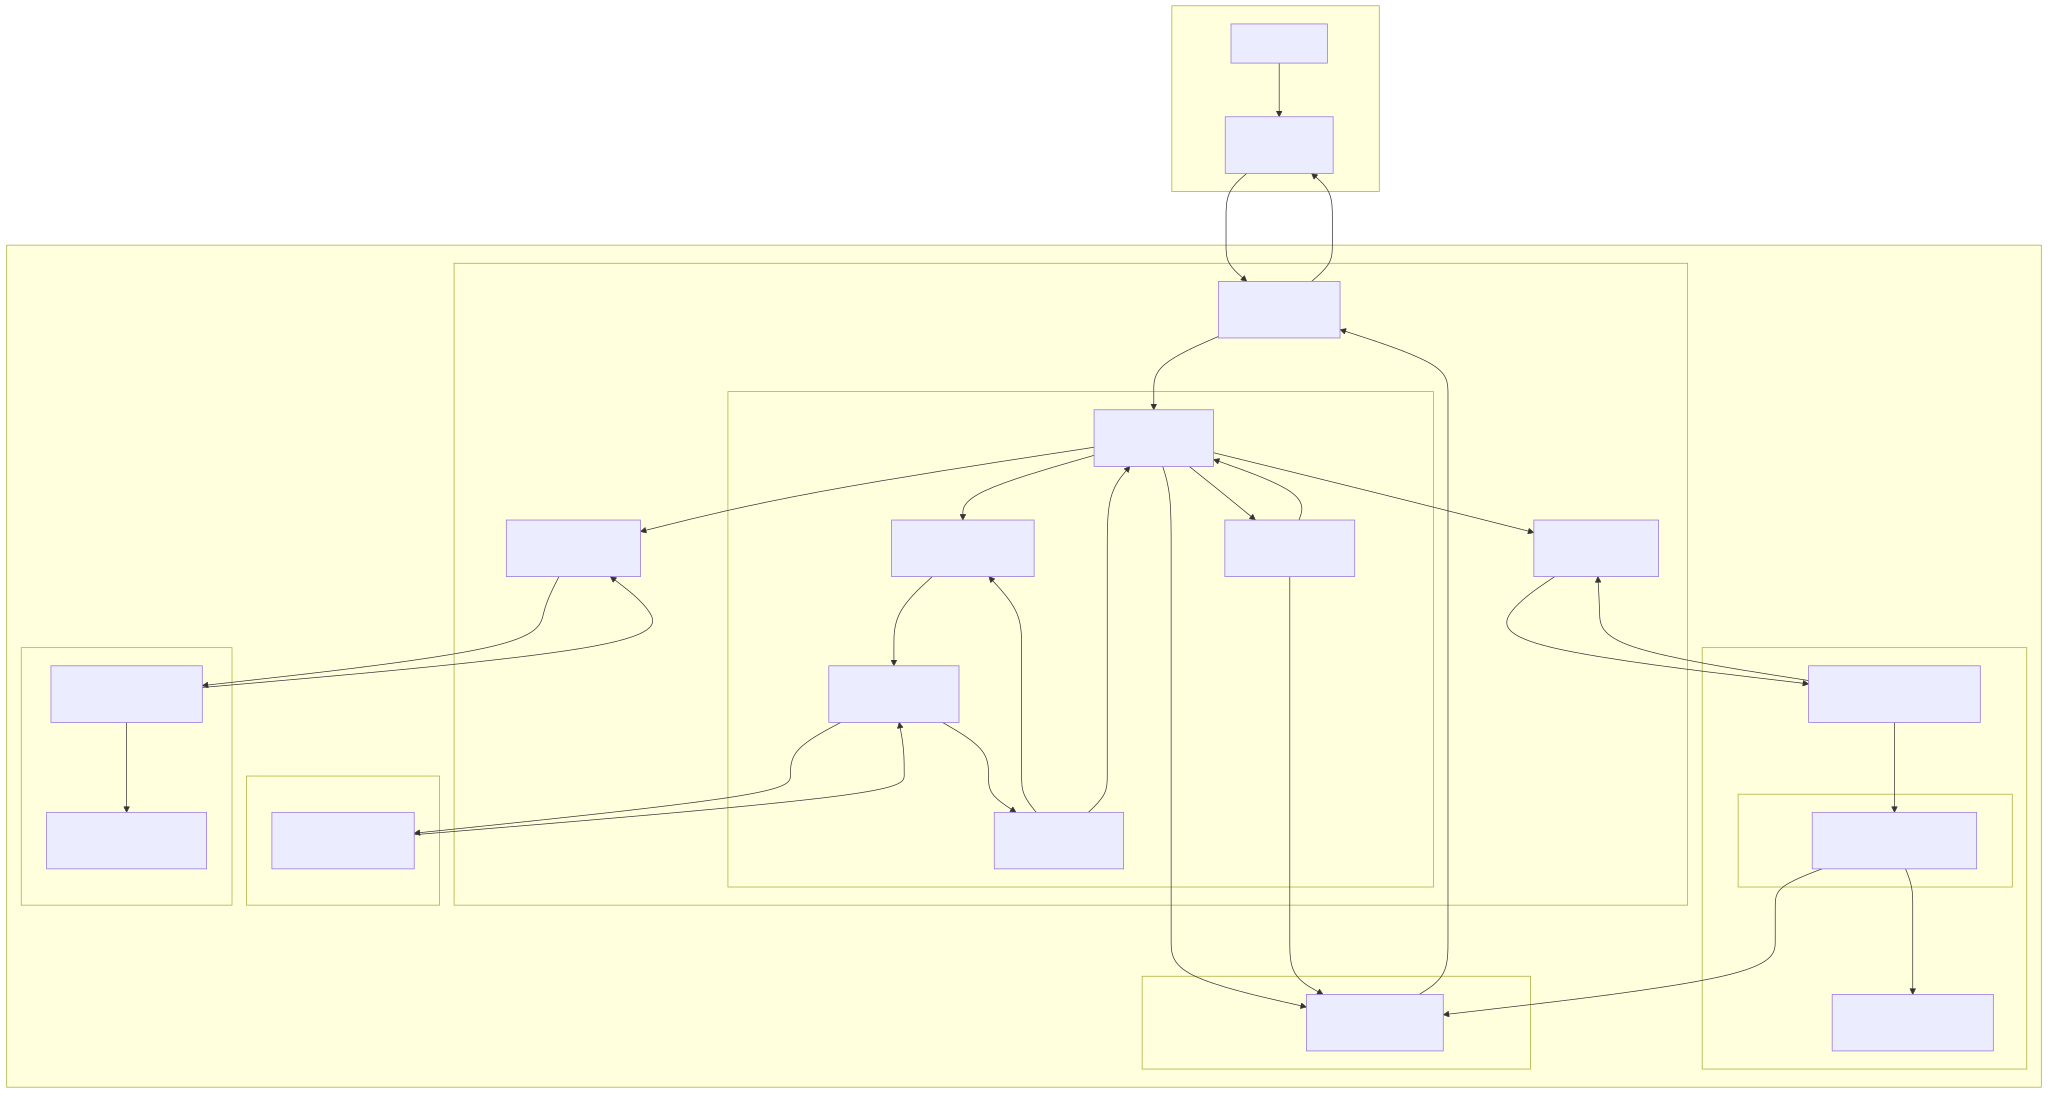
\includegraphics[width = 1.0\textwidth]{static-page/architecture.png}
%     \caption{Cool train station}
%     \label{fig: image}
% \end{figure*}

% \begin{table*}[htbp]
%     \centering
%     \caption{表格範例標題} \label{tab: complexity}
%     \makebox[\linewidth][c]{
%     \renewcommand\arraystretch{1.2}{
%         \begin{tabular}{| l | c  c  c  c |}
%         \hline
%         Protocol & $P$ & $CS_1$ & $CS_2$ & $RG$ \\
%         \hline
%         MSSMul & $O(1)$, $O(1)$, N/A & $O(n-t)$, $O(n)$, $O(1)$ & $O(n-t)$, $O(n)$, N/A & $O(1)$, $O(n)$, $O(n)$ \\
%         SC & $O(1)$, $O(1)$, N/A & $O(n-t)$, $O(n)$, $O(1)$ & $O(n-t)$, $O(n)$, N/A & $O(1)$, $O(n)$, $O(n)$ \\
%         \hline 
%         \end {tabular}
%     }}
% \end {table*}

% \section{模型說明(小標)}

% 說明說明說明說明,說明說明說明說明說明說明說明說明說明說明說明說明,說明說明說明說明說明說明說明說明。

% \begin{figure*}[htbp]
%     \centering
%     \includegraphics[width = 0.5\textwidth]{image.jpeg}
%     \caption{Cool train station}
%     \label{fig: image}
% \end{figure*}

\end{ZhChapter}